\subsection{Recap}
\begin{frame}<12>[b]{\insertsubsection}
	\vspace{-20mm}\small\renewcommand{\projectcartoonwidth}{.18}
	\begin{fancycolumns}[widths={30},animation=none]
		\uncover<11->{\begin{definition}{Why Do Software Projects Fail?}
				\begin{itemize}
					\item many stakeholders with different background each
					\item miscommunication
					\item implicit or wrong assumptions
					\item time pressure
					\item high complexity
					\item \ldots
					\item numerous reasons specific to certain phases and roles
				\end{itemize}
			\end{definition}}
		\uncover<12->{\begin{note}{}\centering{}software engineering aims to\\reduce such problems\end{note}}
		\nextcolumn
		\centering\hprojectcartoon{01}{how the customer explained it} % se02-10 requirements
		\uncover<2->{\hprojectcartoon{02}{how the project leader understood it}} % se02-07 modeling
		\uncover<3->{\hprojectcartoon{03}{how the analyst designed it}} % se04-10 architecture anddesign
		\uncover<4->{\hprojectcartoon{04}{how the programmer implemented it}} % se02-10 implementation
		\uncover<5->{\hprojectcartoon{05}{what the beta testers received}} % se08-09 testing

		\uncover<6->{\hprojectcartoon{06}{how the business consultant described it}} % se02-03 process
		\uncover<7->{\hprojectcartoon{09}{how the customer was billed}} % se10 management and pricing
		\uncover<8->{\hprojectcartoon{10}{how it was supported}} % se12 maintenance
		\uncover<9->{\hprojectcartoon{12}{when it was delivered}} % se13 continous integration/delivery
		\uncover<10->{\hprojectcartoon{13}{what the customer really needed}} % se02-05
		%\hspace{-7mm}
		%\projectcartoon{07}{how the project was documented} % code documentation
		%\hprojectcartoon{18}{how patches were applied} % se11 evolution
		%\hprojectcartoon{17}{how it performed under load} % se14 compilation/quality assurance/performance
		%\hprojectcartoon{11}{what marketing advertised} % se15 reuse/product lines
		%\hprojectcartoon{16}{how open source version} % se16 open source/licensing
		%\projectcartoon{08}{what operations installed} % devops?
		%\projectcartoon{14}{what the digg effect can do to your site} % micro services?
		%\projectcartoon{15}{the disaster recover plan}
		%\hspace{-7mm}
	\end{fancycolumns}
\end{frame}

\subsection{Software Development Process}
\begin{frame}{\insertsubsection}
	\begin{fancycolumns}
		\begin{note}{Motivation}
			\begin{itemize}
				\item how to \emph{structure} the project?
				\item what are \emph{activities} and phases?\\analysis (requirements elicitation + system modeling), design (architectural + software design), implementation, test, deployment
				\item how to organize \emph{communication}?
				\item who has which \emph{responsibilities}?
				\item did we \emph{forget} anything?
				\item can we \emph{predict} the project result?
				\item how to \emph{manage and control} progress?
				\item how to share and elicit \emph{experience}?
				\item how to synchronize \emph{hardware} and software development?
			\end{itemize}
		\end{note}
		\nextcolumn
		\begin{definition}{Software Process Model\mysource{\sommerville}}
			\begin{itemize}
				\item Software process = set of activities related to production of software system
				\item Roles = responsibilities of stakeholders
				\item Software process models = abstract framework for guiding software process, establish roles, provide pre-/post-conditions
			\end{itemize}
		\end{definition}
		\uncover<3->{\begin{note}{Why Different Processes/Models? \mysource{\sommerville}}
				\mycite{The process used in different companies depends on the type of software being developed, the requirements of the software customer, and the skills of the people writing the software.}
			\end{note}}
	\end{fancycolumns}
\end{frame}

\subsection{Categories of Software Process Models}
\begin{frame}
	\frametitle{\insertsubsection{}}

	\begin{fancycolumns}[t]
		\begin{note}{Sequential vs Iterative}
			\begin{itemize}
				\item Sequential (e.g., Waterfall)
				      \begin{itemize}
					      \item Upfront planning; limited changes
					      \item Linear progress through pre-defined phases
				      \end{itemize}
				\item Iterative (e.g., Spiral)
				      \begin{itemize}
					      \item More flexible to changes
					      \item Repeated cycles
				      \end{itemize}
			\end{itemize}
		\end{note}
		\nextcolumn
		\begin{note}{Formal vs Informal}
			\begin{itemize}
				\item Formal (e.g., Spiral)
				      \begin{itemize}
					      \item Fixed set of rules
					      \item Precise specification for verification \& validation
				      \end{itemize}
				\item Informal (e.g., Kanban)
				      \begin{itemize}
					      \item Lightweight framework
					      \item Adaptations according to team practices
				      \end{itemize}
			\end{itemize}
		\end{note}

	\end{fancycolumns}


\end{frame}

% TODO add slide(s) on requirements and design?

\subsection{Waterfall Model}
\begin{frame}{\insertsubsection{} \deutsch{Wasserfallmodell} \mytitlesource{\sommerville}}
	\slideWaterfallModel
\end{frame}

\begin{frame}{\insertsubsection\ \mytitlesource{\sommerville}}
	\begin{fancycolumns}[animation=none]
		\begin{definition}{1. Requirements Analysis}
			\mycite{The system’s services, constraints, and goals are established by consultation with system users. They are then defined in detail and serve as a \emph{system specification}.}
		\end{definition}
		\begin{definition}{2. System and Software Design}
			\mycite{The systems design process allocates the requirements to either hardware or software systems. It establishes an overall \emph{system architecture}. Software design involves identifying and describing the fundamental software system abstractions and their relationships.}
		\end{definition}
		\nextcolumn
		\vspace{-11mm}
		\begin{definition}{3. Implementation and Unit Testing}
			\mycite{During this stage, the software design is realized as a set of \emph{programs or program units}. Unit testing involves verifying that each unit meets its specification.}
		\end{definition}
		\begin{definition}{4. Integration and System Testing}
			\mycite{The individual program units or programs are integrated and tested as a complete system to ensure that the software requirements have been met. After testing, the \emph{software system is delivered} to the customer.}
		\end{definition}
		\begin{definition}{5. Operation and Maintenance}
			\mycite{Normally, this is the longest life-cycle phase. The system is installed and put into practical use. Maintenance involves \emph{correcting errors} that were not discovered in earlier stages of the life cycle [...].%, improving the implementation of system units, and enhancing the system’s services as new requirements are discovered.
			}
		\end{definition}
	\end{fancycolumns}
\end{frame}

\begin{frame}{\insertsubsection{} -- Examples\ \mytitlesource{\sommerville}}
	\begin{fancycolumns}[animation=none]
		\begin{example}{Example Domains}
			\begin{itemize}
				\item \emph{embedded systems} where software has to interface with hardware systems
				\item \emph{critical systems} with extensive safety and security analysis of specification and design
				\item \emph{large software systems} that are typically developed by several companies
			\end{itemize}
		\end{example}
		\nextcolumn
		\pic[width=\linewidth]{misc/lawn-mower-cropped}
	\end{fancycolumns}
\end{frame}

\begin{frame}{\insertsubsection{} -- Discussion\ \mytitlesource{\sommerville}}
	\begin{fancycolumns}
		\begin{note}{Advantages}
			\begin{itemize}
				\item easy to understand, manage, and control
				\item good for systems development (i.e., with high manufacturing costs for hardware)
				\item easier to use the same model as for hardware
				\item combination with formal system development feasible (e.g., B method)
			\end{itemize}
		\end{note}
		\nextcolumn
		\begin{note}{Disadvantages}
			\begin{itemize}
				\item for software development: stages should feed information to each other
				\item changes in previous stages are hard to achieve
				\item problems from previous stages left for later resolution
				\item freezing of requirements may lead to software not wanted by the user
				\item freezing of design may lead to bad structure and implementation tricks
				\item requires clear and stable requirements and good design upfront
			\end{itemize}
		\end{note}
	\end{fancycolumns}
\end{frame}

% TODO explain the difference between requirements elicitation and system model + architecture design vs software design

\subsection{V-Model}
\begin{frame}{\insertsubsection}
	\begin{fancycolumns}
		\begin{definition}{V-Model \mysource{\ludewiglichter}}
			\begin{itemize}
				\item sequential \& formal
				\item developed by the German Ministry of Defense \deutsch{Verteidigungsministerium} and required since 1992
				\item extension of the waterfall model: project-aligned activities such as quality assurance, configuration management, project management
				\item 1997 V-model 97: incremental development, inclusion of hardware, object-oriented development
				\item 2004 V-model XT (for extreme tailoring): adaptability, application beyond software
				      % four project types of V-model XT
				\item integration of four testing stages
				      %\item distinction between validation (right product) and verification (product correct)
				      % fake? proposed 1979 by Barry Boehm
			\end{itemize}
		\end{definition}
		\nextcolumn
		\diagramVModel
		% TODO find reference for this kind of V model
	\end{fancycolumns}
\end{frame}

\subsection{Stages of Testing}
\begin{frame}{\insertsubsection\ \deutsch{Teststufen}\ \mytitlesource{\ludewiglichter, \sommerville}}
	\slideStagesTesting
\end{frame}
% TODO split on several slides and give examples for errors that should / should not be found in this phase (and why)

\begin{frame}{V-Model -- Examples\ \mytitlesource{\ludewiglichter}}
	\begin{fancycolumns}[animation=none]
		\begin{example}{Example Domains}
			\begin{itemize}
				\item since 1992 V-model required by German government (e.g., Bundeswehr), since 2004 V-model XT
				\item embedded, critical, and large software systems as for the waterfall model
			\end{itemize}
		\end{example}
		\nextcolumn
		\pic[width=\linewidth]{misc/lawn-mower-cropped}
		% TODO picture associated with German government?
	\end{fancycolumns}
\end{frame}

\begin{frame}{V-Model -- Discussion\ \mytitlesource{\ludewiglichter}}
	\begin{fancycolumns}
		\begin{note}{Advantages}
			\begin{itemize}
				\item quality assurance in several testing stages
				\item completeness helps to not miss activities
				      %\item distinction between validation and verification
				\item V-model 97/XT are widely applicable (e.g., hardware, incremental)
			\end{itemize}
		\end{note}
		\nextcolumn
		\begin{note}{Disadvantages}
			\begin{itemize}
				\item complex and extensive process
				\item adaptations often required (cf.\ XT for extreme tailoring)
				\item overhead useful only for large software systems
				\item changes in requirements are problematic
			\end{itemize}
		\end{note}
	\end{fancycolumns}
\end{frame}

% filepath: /home/chicosundermann/git/teaching/se2/Course-on-Software-Engineering/se1/content/05b-processmodels.tex
% ...existing code...

\subsection{Spiral Model}
\begin{frame}{\insertsubsection\ \mytitlesource{\sommerville}}
    \begin{fancycolumns}[animation=none]
        \begin{definition}{Core Idea}
            \begin{itemize}
                \item iterative, formal 
				\item risk-driven development
                \item each loop represents one development cycle
                \item run through four main tasks in each cycle: set objectives, address risks, develop an increment, and plan the next loop
                \item prototypes in each cycle help explore alternatives and reduce risk
                \item each loop expands the system toward an operational product
            \end{itemize}
        \end{definition}
        \nextcolumn
        \centering
        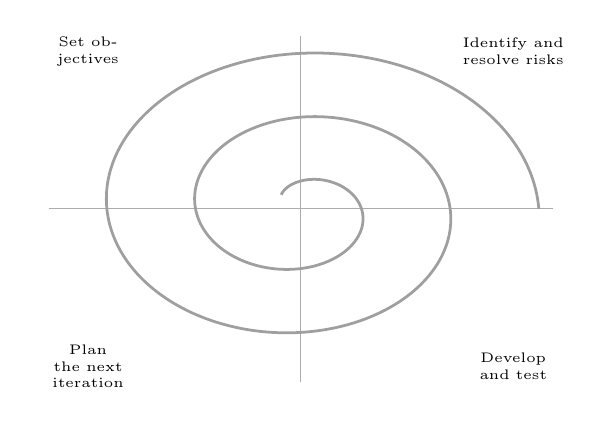
\begin{tikzpicture}[>=stealth]


            % Axes
            \draw[gray!65] (-3.2,0) -- (3.2,0);
            \draw[gray!65] (0,-2.2) -- (0,2.2);

            % Expanding spiral, starting in the upper-left quadrant
            \draw[gray!75, line width=1pt, samples=500, domain=0:855,
                variable=\t]
                plot ({(0.35+0.00313*\t)*cos(135-\t)},
                      {0.72*(0.35+0.00313*\t)*sin(135-\t)});

            % Activities around the spiral
            \node[font=\tiny, align=center, text width=1.3cm] at (-2.7,2)
                {Set objectives};
            \node[font=\tiny, align=center, text width=1.3cm] at (2.7,2)
                {Identify and resolve risks};
            \node[font=\tiny, align=center, text width=1.3cm] at (2.7,-2)
                {Develop and test};
            \node[font=\tiny, align=center, text width=1.3cm] at (-2.7,-2)
                {Plan the next iteration};
        \end{tikzpicture}
    \end{fancycolumns}
\end{frame}

\begin{frame}{\insertsubsection{} -- Activities\ \mytitlesource{\sommerville}}
    \begin{fancycolumns}[animation=none]
        \begin{definition}{1. Set Objectives}
            \begin{itemize}
                \item define goals for this cycle
                \item identify alternatives and constraints
            \end{itemize}
        \end{definition}
        \begin{definition}{2. Assess and Reduce Risks}
            \begin{itemize}
                \item identify the cycle's key risks
                \item use prototypes or analysis to address them
            \end{itemize}
        \end{definition}
        \nextcolumn
        \begin{definition}{3. Develop and Verify}
            \begin{itemize}
                \item build the next system increment
                \item evaluate it against the cycle's objectives
            \end{itemize}
        \end{definition}
        \begin{definition}{4. Plan the Next Cycle}
            \begin{itemize}
                \item review results with stakeholders
                \item choose objectives and an approach for the next cycle
            \end{itemize}
        \end{definition}
    \end{fancycolumns}
\end{frame}

\begin{frame}{\insertsubsection{} -- Discussion\ \mytitlesource{\sommerville}}
	\begin{fancycolumns}
		\begin{note}{Advantages}
			\begin{itemize}
				\item risks are identified and addressed early
				\item accommodates changing requirements and priorities
				\item prototypes and increments support regular feedback
				\item suitable for large, complex, or high-risk projects
			\end{itemize}
		\end{note}
		\nextcolumn
		\begin{note}{Disadvantages}
			\begin{itemize}
				\item risk assessment requires expertise
				\item planning and review can add significant overhead
				\item progress, cost, and completion dates can be harder to predict
				\item may be unsuitable for small or low-risk projects
			\end{itemize}
		\end{note}
	\end{fancycolumns}
\end{frame}

% ...existing code...

